\section{Experiments}


%\iffalse 
\begin{table*}[t]
\centering
\begin{tabular}{c|c|c|c|c|c||c|c|c}
\toprule
\multirow{2}{*}{Backbone} &    \multirow{2}{*}{Method} & \multicolumn{4}{c||}{ID: Pascal} & \multicolumn{3}{c}{ID: Cityscapes}  \\
 &           & Comic & Watercolor & Clipart & ID                           & Foggy & BDD  & ID    \\\hline
\multirow{4}{*}{ResNet50 Instagram~\cite{mahajan2018exploring}}&DP                                   & 15.7  & 21.2       & 15.3    & 44.6 &                                    13.9 & 7.7 & 28.3  \\
&FT                                   & 7.5   & 19.4       & 11.4    & 50.4 &                                     12.8  & 5.1  & 33.5 \\
%&FT + Augmix                          & 10.2  & 21.9       & 12.4    & 46.3 &                                    &       &             \\
& \CCG DP-FT                                &\CCG 9.1   & \CCG21.0       & \CCG12.9    &\CCG 52.6 &\CCG14.8  &\CCG 5.5  &\CCG\bf{34.7}  \\
 &\CCG DP-FT + WR           &\CCG \bf{16.8}  &\CCG \bf{26.5}       &\CCG \bf{17.6}    &\CCG \bf{52.9} &\CCG \bf{19.3}  &\CCG \bf{9.6}  &\CCG 34.5   \\\hline
 %&\CCG All                &\CCG \bf{18.9}  &\CCG \bf{27.5}       &\CCG \bf{21.4}    &\CCG 52.2 &\CCG  \\\hline                                     
\multirow{4}{*}{ConvNeXt IN21K~\cite{liu2022convnet}}&DP                                   & 11.7  & 17.3       & 14.0    & 39.7 &                                     14.7 & 7.8 & 31.1 \\
&FT                              &      11.5  & 22.9       & 16.8    & 60.6 &  18.1 & 9.7 & 35.8    \\
%&FT + Augmix                  &         15.5  & 28.6       & 20.7    & 61.4 &                                    &      &             \\
&\CCG  DP-FT                   & \CCG              13.6  &\CCG  24.7       &\CCG  19.1    &\CCG  \bf{62.3} & \CCG                                   20.5&\CCG 11.5&\CCG   37.1\\
%&\CCG  DP-FT + Seblock         &\CCG               15.4  &\CCG  27.5       &\CCG  20.9    &\CCG  61.6 &\CCG   \bf{22.0}  &\CCG  11.3 &\CCG  36.6            \\
&\CCG DP-FT + WR     &\CCG       \bf{14.6}  &\CCG  \bf{27.8}       &\CCG  \bf{19.7}    &\CCG  61.4 & \CCG                          \textbf{21.1}          &\CCG    \textbf{11.7}     &\CCG  \bf{37.2}   \\\hline
%&\CCG  All              &\CCG   \bf{17.8}  &\CCG  \bf{29.3}       &\CCG  \bf{23.8}    &\CCG  \bf{61.0}   &\CCG  21.7&\CCG  \bf{11.8}&\CCG  37.2            \\\hline
%&DP-FT + Reg + Augmix & 21.0  & 27.9       & 22.6    & 50.4 &            \\    \hline
\multirow{4}{*}{Eff-B2 JFT~\cite{xie2020self}}&  DP                                   & 12.6  & 20.4       & 15.1    & 40.2 &                                     11.1 & 6.9 & 25.2 \\
&FT                                   & 17.1  & 27.2       & 18.0    & 53.4 &          10.7                          &  5.1     &     31.5        \\
%&FT + Augmix                          & 20.1  & 31.2       & 19.7    & 52.7 &                                    &       &             \\
&\CCG  DP-FT                                &\CCG  17.4  &\CCG  29.4       &\CCG  20.7    &\CCG \bf{55.3} &\CCG   12.9&\CCG  7.3&\CCG   \bf{32.9}\\
&\CCG  DP-FT + WR        &\CCG  \bf{19.5}  &\CCG  \bf{30.0}         &\CCG  \bf{22.0}      &\CCG  54.2 &\CCG \bf{13.5} &\CCG  \bf{7.6} &\CCG  32.5\\

% \bf{13.1}&\CCG  \bf{7.5}&\CCG  32.7\\
\bottomrule
\end{tabular}
\vspace{-3mm}
\caption{Effect of weight regularization. DP, FT, and WR denote decoder-probing, fine-tuning, and weight regularization.} 
\label{tb:main}
\end{table*}

\iffalse 

\begin{table*}[]
\centering
\begin{tabular}{c|c|c|c|c|c|c}
\toprule
 \multirow{1}{*}{Backbone} &    \multirow{1}{*}{Method}           & Comic & Watercolor & Clipart & OOD Average& ID: Pascal          \\\hline
\multirow{6}{*}{ResNet50 Instagram}&DP                                   & 15.7  & 21.2       & 15.3    & 17.4&44.6   \\
&FT                                   & 7.5   & 19.4       & 11.4    & 12.8&50.4 \\
%&FT + Augmix                          & 10.2  & 21.9       & 12.4    & 46.3 &                                    &       &             \\
& \CCG DP-FT                                &\CCG 9.1   & \CCG21.0       & \CCG12.9  &\CCG 14.3  &\CCG 52.6 \\
&\CCG DP-FT + Seblock                      &\CCG 10.2  & \CCG 22.5       &\CCG 15.1    &\CCG 15.9 & \CCG \bf{53.4} \\
 &\CCG DP-FT + Reg           &\CCG 16.8  &\CCG 26.5       &\CCG 17.6    &\CCG 19.9&\CCG 52.9 \\
 &\CCG All                &\CCG \bf{18.9}  &\CCG \bf{27.5}       &\CCG \bf{21.4} & \CCG \bf{22.6} &\CCG 52.2 \\\hline                                     
\multirow{6}{*}{Convnext IN21K}&DP                                   & 11.7  & 17.3       & 14.0    & 14.3&39.7 \\
&FT                              &      11.5  & 22.9       & 16.8    &17.1& 60.6    \\
%&FT + Augmix                  &         15.5  & 28.6       & 20.7    & 61.4 &                                    &      &             \\
&\CCG  DP-FT                   & \CCG              13.6  &\CCG  24.7       &\CCG  19.1    &\CCG19.1&\CCG  62.3 \\
&\CCG  DP-FT + Seblock         &\CCG               15.4  &\CCG  27.5       &\CCG  20.9    &\CCG 21.3&\CCG  61.6 \\
&\CCG DP-FT + Reg     &\CCG       14.6  &\CCG  27.8       &\CCG  19.7    &\CCG20.7&\CCG  61.4 \\
&\CCG  All              &\CCG   \bf{17.8}  &\CCG  \bf{29.3}       &\CCG23.6&\CCG  \bf{23.8}    &\CCG  \bf{61.0}   \\\hline
%&DP-FT + Reg + Augmix & 21.0  & 27.9       & 22.6    & 50.4 &            \\    \hline
\multirow{4}{*}{Eff-B2 JFT}&  DP                                   & 12.6  & 20.4       & 15.1    &  16.0&40.2 \\
&FT                                   & 17.1  & 27.2       & 18.0    &20.8& 53.4 \\
%&FT + Augmix                          & 20.1  & 31.2       & 19.7    & 52.7 &                                    &       &             \\
&\CCG  DP-FT                                &\CCG  17.4  &\CCG  29.4       &\CCG  20.7    &\CCG 22.5&\CCG  \bf{55.3} \\
&\CCG  DP-FT + WR        &\CCG  \bf{19.5}  &\CCG  \bf{30.0}         &\CCG  \bf{22.0}      &\CCG 23.8&\CCG  54.2 \\
\bottomrule
\end{tabular}
\caption{Improvements by introducing our proposed modules.}
\label{tb:main}
\end{table*}
\fi

%\fi


\iffalse 
\begin{table*}[]
\centering
\begin{tabular}{c|c|c|c|c|c||c|c|c}
\toprule
\multirow{2}{*}{Model} &    \multirow{2}{*}{Method} & \multicolumn{4}{c||}{ID: Pascal} & \multicolumn{3}{c}{ID: Cityscape}  \\\cline{3-9}
 &           & Comic & Watercolor & Clipart & ID                           & Foggy & BDD  & ID    \\\hline
\multirow{6}{*}{ResNet50 Instagram}&DP                                   & 15.7  & 21.2       & 15.3    & 44.6 &                                    13.9 & 7.66 & 28.3  \\
&FT                                   & 7.5   & 19.4       & 11.4    & 50.4 &                                     12.8  & 5.1  & 33.52 \\
%&FT + Augmix                          & 10.2  & 21.9       & 12.4    & 46.3 &                                    &       &             \\
& \CCG DP-FT                                &\CCG 9.1   & \CCG21.0       & \CCG12.9    &\CCG 52.6 &\CCG14.8  &\CCG 5.5  &\CCG34.7  \\
&\CCG DP-FT + SE                      &\CCG 10.2  & \CCG 22.5       &\CCG 15.1    &\CCG \bf{53.4} &\CCG                                    &\CCG       &\CCG             \\
 &\CCG DP-FT + WR           &\CCG 16.8  &\CCG 26.5       &\CCG 17.6    &\CCG 52.9 &\CCG \bf{19.3}  &\CCG \bf{9.6}  &\CCG 34.5   \\
 &\CCG All                &\CCG \bf{18.9}  &\CCG \bf{27.5}       &\CCG \bf{21.4}    &\CCG 52.2 &\CCG  \\\hline                                     
\multirow{6}{*}{Convnext IN21K}&DP                                   & 11.7  & 17.3       & 14.0    & 39.7 &                                     14.7 & 7.8 & 31.1 \\
&FT                              &      11.5  & 22.9       & 16.8    & 60.6 &  18.1 & 9.7 & 35.8    \\
%&FT + Augmix                  &         15.5  & 28.6       & 20.7    & 61.4 &                                    &      &             \\
&\CCG  DP-FT                   & \CCG              13.6  &\CCG  24.7       &\CCG  19.1    &\CCG  62.3 & \CCG                                   20.5&\CCG 11.5&\CCG  37.1\\
&\CCG  DP-FT + Seblock         &\CCG               15.4  &\CCG  27.5       &\CCG  20.9    &\CCG  61.6 &\CCG   \bf{22.0}  &\CCG  11.3 &\CCG  36.6            \\
&\CCG DP-FT + Reg     &\CCG       14.6  &\CCG  27.8       &\CCG  19.7    &\CCG  61.4 & \CCG           20.9                         &\CCG   11.8     &\CCG  \bf{37.5}             \\
&\CCG  All              &\CCG   \bf{17.8}  &\CCG  \bf{29.3}       &\CCG  \bf{23.8}    &\CCG  \bf{61.0}   &\CCG  21.7&\CCG  \bf{11.8}&\CCG  37.2            \\\hline
%&DP-FT + Reg + Augmix & 21.0  & 27.9       & 22.6    & 50.4 &            \\    \hline
\multirow{4}{*}{Eff-B2 JFT}&  DP                                   & 12.6  & 20.4       & 15.1    & 40.2 &                                     11.1 & 6.9 & 25.2 \\
&FT                                   & 17.1  & 27.2       & 18.0    & \bf{53.4} &          10.7                          &  5.1     &     31.5        \\
%&FT + Augmix                          & 20.1  & 31.2       & 19.7    & 52.7 &                                    &       &             \\
&\CCG  DP-FT                                &\CCG  17.4  &\CCG  29.4       &\CCG  20.7    &\CCG  55.3 &\CCG   12.9&\CCG  7.3&\CCG   \bf{32.9}\\
&\CCG  DP-FT + Reg        &\CCG  \bf{19.5}  &\CCG  \bf{30.0}         &\CCG  \bf{22.0}      &\CCG  54.2 &\CCG  \bf{13.1}&\CCG  \bf{7.5}&\CCG  32.7\\
\bottomrule
\end{tabular}
\caption{Improvements by Applying weight regularization.}
\label{tb:main}
\end{table*}
\fi

\subsection{Experimental Settings}

\textbf{Datasets} We evaluate our approach on MuST-C V1 English-German (EnDe), English-Spanish (EnEs) and English-French (EnFr) datasets \citep{di-gangi-etal-2019-must}, 
where limited previous works discussed the En-Fr streaming ST with BLEU-latency curve. 
All the corpora contain source audios, source transcriptions, and target translations, and the results reported are conducted on the corresponding tst-COMMON set. 
Detailed statistics of different language pairs are given in Appendix \ref{apd:data_statistics}.

For speech data, we normalize the raw audio wave to the range of $[-1,1)$. 
For text data, we keep punctuation and remove non-printing characters, and remain case-sensitive. 
For each translation direction, the unigram SentencePiece\footnote{\url{https://github.com/google/sentencepiece}} model \citep{kudo-richardson-2018-sentencepiece} is used to learn a shared vocabulary of size 10k. 
\\
\textbf{Model Configuration} 
For the acoustic encoder, we use Wav2vec2.0\footnote{\url{https://dl.fbaipublicfiles.com/fairseq/wav2vec/wav2vec\_small.pt}} \citep{NEURIPS2020_92d1e1eb} following the base configurations. 
We construct the acoustic boundary detector by applying the CIF \citep{yi2021efficiently} on the last dimension of speech representation. 
We use 8 and 6 layers for the semantic encoder and the translation decoder respectively, with 4 attention heads and 768 hidden units.
\\
\textbf{Training} 
The detailed training schedule of the offline ST model is given in Appendix \ref{apd:details_of_training}. 
We set the length $m$ of future context tokens to 50 for both FAD and FAI. 
All hyper-parameters are tuned on EnDe devset and applied to other language pairs. 
We train all models with 3.2 million frames per batch on 8 Nvidia Tesla V100 GPUs. 
We implement our models with Fairseq\footnote{\url{https://github.com/pytorch/fairseq}} \cite{ott-etal-2019-fairseq}.
\\
\textbf{Inference} We average the checkpoints of the best 10 epochs on development set for evaluation. 
We perform streaming-testing with the \textit{wait-$k$} policy. 
$k$ is counted by the detected acoustic units from the CIF module. 
To follow the tradition in simultaneous translation \citep{zeng-etal-2021-realtrans,dong-etal-2022-learning}, we do not rewrite the tokens that have already been generated. 
\\
\textbf{Evaluation Metrics} We use SacreBLEU\footnote{\url{https://github.com/mjpost/sacrebleu}} for the translation quality. 
The latency is evaluated with Average Latency (AL) \citep{ma-etal-2019-stacl}, Average Proportion (AP) \citep{cho2016can}, and Differentiable Average Lagging (DAL) \citep{cherry2019thinking} in the SimulEval\footnote{\url{https://github.com/facebookresearch/SimulEval}} \citep{ma-etal-2020-simuleval}. 
\\
\textbf{System Settings} 
We compare our method with several strong end-to-end streaming ST approaches. 
(\romannumeral1) \textit{SimulSpeech} \citep{ren-etal-2020-simulspeech} and \textit{RealTranS} \citep{zeng-etal-2021-realtrans} use uni-directional encoder rather than bidirectional one. 
(\romannumeral2) \textit{MoSST} \citep{dong-etal-2022-learning} applies an offline-trained model with a monotonic segmentation module for streaming testing and achieves competitive performance. 
(\romannumeral3) \textit{MMA-SLM} \cite{indurthi-etal-2022-language} enhances monotonic attention to make better read/write decisions by integrating future information from language models.
(\romannumeral4) \textit{ITST} \cite{zhang-feng-2022-information} learns an adaptive read/write policy by quantifying the transported information weight from source token to the target token.
(\romannumeral5) \textit{MU-ST} \citep{zhang-etal-2022-learning} learns an adaptive segmentation policy to detect meaningful units, which makes read/write decisions. 
(\romannumeral6) \textit{Baseline} is our offline-trained ST model (\textbf{B} for abbreviation). 
For fair comparisons, it has the same structure as MoSST. 




\subsection{Main Results}

We presents the main results in Figure \ref{fig:main_results} \footnote{The extended results for other latency metrics (AP and DAL) are described in Appendix \ref{apd:appendix_more_results}.}. 
Compared with the online models SimulSpeech, RealTranS, and ITST, our offline model (baseline) achieves higher translation quality with high latency as it encodes bidirectional context information during training, however, in the low latency region, it performs poorly due to the input mismatch between offline-training and online-decoding. 

\textbf{B + FAI} With the ability to reduce this mismatch, FAI is directly applied for our offline (baseline) model and can achieve higher BLEU in all latency regions. 
In particular, it outperforms our most compatible baseline \textbf{B} by large margins in lower latency regions (when AL is less than 1000\emph{ms}), with improvements over 6 BLEU in both EnDe and EnEs, 10 BLEU in EnFr.

\textbf{FAST} (FAD + FAI) Furthermore, our FAST achieves the best trade-off between translation quality and latency, especially at extremely low latency region (AL is about 200\emph{ms}, $k=1$), achieving the improvements of 6 BLEU in EnDe, 10 BLEU in EnEs, and 4 BLEU in EnFr compared to B + FAI.
It indicates that FAST can effectively mitigate the input mismatch between offline-training and online-decoding.
In addition, our method achieves comparable translation quality with full-speech translation at middle latency (at AL around 3000\emph{ms}), especially for EnEs.


\subsection{Ablation Study}
\label{sec:ablation}

\begin{figure}[t]
\centering
\includegraphics[width=1.0\linewidth]{ablation.pdf}
\caption{Ablation study of our method on the tst-COMMON set of MuST-C EnDe dataset. The observed points in the plots represent wait-$k$ policy with $k=\{1,3,5,7,9,12,15,20,30\}$.}
\label{fig:ablation}
\end{figure}

In this section, we study the effectiveness of our methods. 
All ablation results are obtained from the MuST-C EnDe tst-COMMON set. 
The results are shown in Figure \ref{fig:ablation}.

(1) \textit{w/o $\mathcal{L}_{KD}^{\text{W2V2}}$}: if removing the $\mathcal{L}_{KD}^{\text{W2V2}}$, the translation quality drops by 1-2 BLEU in all latency regions, including high latency region.
This demonstrates optimizing $\mathcal{L}_{KD}^{\text{W2V2}}$ can guarantee the full speech translation performance.

(2) \textit{w/o $\mathcal{L}_{KD}^{\text{CIF}}$}: If removing the $\mathcal{L}_{KD}^{\text{CIF}}$, the translation quality will be slightly degraded. 
However, we observe that the distances between two consecutive acoustic boundaries become larger. 
For example, the AL of this variant at \textit{wait-1} is greater than 750, but the AL of the other variants at \textit{wait-1} is approximately 150. 
As expected, optimizing $\mathcal{L}_{KD}^{\text{CIF}}$ can ensure the correct acoustic boundaries.

(3) \textit{w/o FAI}: In this variant, we use the student model by FAD with vanilla \textit{wait-k} policy for streaming inference (\emph{i.e.}, inference without mask tokens). 
However, FAD training considers mask tokens as student input, so this mismatch leads to significant performance degradation in low and middle latency regions.  
This indicates that our FAD and FAI should be used together to achieve better streaming performance.

(4) \textit{w/o mask embeddings}: During training and inference, our model appends $m$ mask tokens into streaming speech tokens as the pseudo future contexts. 
In this variant, we remove the mask tokens during both training and inference. 
Even though no mismatch, we still observe a significant drop in translation quality, especially for high latency. 
This result indicates that the pseudo future contexts can enhance the streaming speech representations.

\subsection{How much future context is needed?}

\definecolor{cycle1}{HTML}{1f77b4}
\definecolor{cycle2}{HTML}{ff7f0e}
\definecolor{cycle3}{HTML}{2ca02c}
\definecolor{cycle4}{HTML}{d62728}
\definecolor{cycle5}{HTML}{9467bd}
\definecolor{cycle6}{HTML}{8c564b}
\definecolor{cycle7}{HTML}{e377c2}
\definecolor{cycle8}{HTML}{7f7f7f}
\definecolor{cycle9}{HTML}{bcbd22}
\definecolor{cycle10}{HTML}{17becf}

\begin{figure}[t]
\centering
\includegraphics[width=1.0\linewidth]{length_bleu.pdf}
\caption{Effect on BLEU-AL curve of FAST w.r.t. $m$.} 
\label{fig:length_bleu}
\end{figure}

\begin{figure}[t]
\centering
\pgfplotsset{width=8.1cm,height=5.5cm,
    every axis y label/.append style={at={(-0.1,0.5)}},
    every axis/.append style={line width=0.6pt},
}
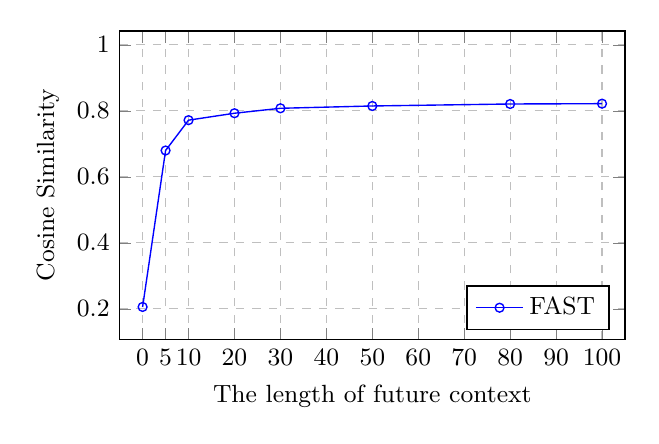
\begin{tikzpicture}[baseline]
\begin{axis}[
    ylabel=Cosine Similarity,
    xlabel=The length of future context,
    enlargelimits=0.05,
    legend pos=south east,
    legend style={font=\small},
    font=\small,
    ymajorgrids=true,
    xmajorgrids=true,
    grid style=dashed,
    ymin=0.15, ymax = 1.0,
    xtick={0,5,10,20,30,40,50,60,70,80,90,100},
]
\addplot[color=blue,mark=o, mark size=1.6pt,line width=0.5pt] coordinates{(0,0.206)(5,0.68)(10,0.772)(20,0.793)(30,0.808)(50,0.815)(80,0.821)(100,0.822)};
\legend{FAST,FAI}
\end{axis}
\end{tikzpicture}
\caption{Effect on the $\Bar{s}_{-1}$ w.r.t. $m$.}
\label{fig:length_cos}
\end{figure}

To answer this question, we explore the FAST (FAD + FAI) with different lengths of future context. 
Figure \ref{fig:length_bleu} shows the overall results. %in $\{0,10,20,30,40,50,60,70\}$
$m=0$ means the offline system without distillation. 
The offline system inherits the mismatch problem, but our method gradually improves the performance as $m$ increasing from 0 to 20. 
Since we found only the representation of last 10 positions is poor (in Section \ref{sec:analysis}), FAST obtains similar BLEU-AL curve when $m$ is significantly larger than 10, \emph{e.g.}, 20-100. 

After the FAD training, we investigate the representation of the last position (before mask tokens) by $\bar{s}_{-1}$ in Eq.~(\ref{eq:audio_cos2}) w.r.t. $m$. 
The results are shown in Figure \ref{fig:length_cos}.
We observe that 1) as $m$ increases, the streaming speech representation of the last position becomes better; 
2) the curves of the cosine similarity becomes flattened when $m > 10$ significantly. 
This is consistent with the trend in Figure \ref{fig:length_bleu}.


\subsection{Analysis on The Representation Gap}

\definecolor{poscolor4}{HTML}{38ada9}
\definecolor{poscolor5}{HTML}{78e08f}
\definecolor{poscolor6}{HTML}{b8e994}
\definecolor{poscolor7}{HTML}{008BCC}
\definecolor{poscolor8}{HTML}{00AC53}
\definecolor{poscolor9}{HTML}{3E4372}
\begin{figure}[t]
\centering
\pgfplotsset{
    width=8cm,height=5.5cm,
    every axis y label/.append style={at={(-0.1,0.5)}},
    every axis/.append style={line width=0.6pt},
}

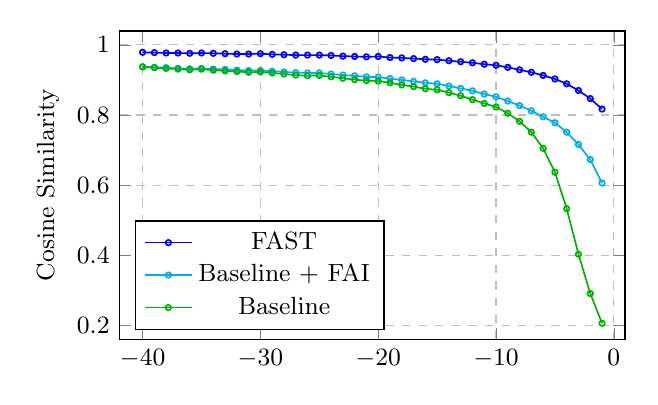
\begin{tikzpicture}[baseline]
\begin{axis}[
    ylabel=Cosine Similarity,
    enlargelimits=0.05,
    font=\small,
    legend pos=south west,
    legend style={font=\small},
    ymajorgrids=true,
    xmajorgrids=true,
    grid style=dashed,
    ymin=0.2, ymax = 1.0,
    ytick={0.2,0.4,0.6,0.8,1.0},
]
\addplot[color=blue,mark=o, mark size=1pt] coordinates{(-40,0.979)(-39,0.978)(-38,0.977)(-37,0.977)(-36,0.976)(-35,0.977)(-34,0.976)(-33,0.975)(-32,0.974)(-31,0.974)(-30,0.975)(-29,0.973)(-28,0.972)(-27,0.971)(-26,0.971)(-25,0.971)(-24,0.97)(-23,0.968)(-22,0.967)(-21,0.966)(-20,0.967)(-19,0.964)(-18,0.963)(-17,0.961)(-16,0.959)(-15,0.958)(-14,0.955)(-13,0.952)(-12,0.949)(-11,0.945)(-10,0.942)(-9,0.936)(-8,0.929)(-7,0.922)(-6,0.913)(-5,0.903)(-4,0.889)(-3,0.87)(-2,0.847)(-1,0.817)};
\addplot[color=cyan,mark=o, mark size=1pt] coordinates{(-40,0.938)(-39,0.936)(-38,0.935)(-37,0.933)(-36,0.932)(-35,0.933)(-34,0.931)(-33,0.930)(-32,0.928)(-31,0.927)(-30,0.927)(-29,0.925)(-28,0.923)(-27,0.921)(-26,0.920)(-25,0.920)(-24,0.917)(-23,0.914)(-22,0.912)(-21,0.909)(-20,0.908)(-19,0.904)(-18,0.900)(-17,0.896)(-16,0.892)(-15,0.889)(-14,0.883)(-13,0.876)(-12,0.869)(-11,0.860)(-10,0.852)(-9,0.840)(-8,0.827)(-7,0.812)(-6,0.795)(-5,0.778)(-4,0.751)(-3,0.716)(-2,0.673)(-1,0.606)};
\addplot[color=green!70!black,mark=o, mark size=1pt] coordinates{(-40,0.937)(-39,0.935)(-38,0.933)(-37,0.931)(-36,0.929)(-35,0.931)(-34,0.928)(-33,0.926)(-32,0.924)(-31,0.922)(-30,0.923)(-29,0.920)(-28,0.917)(-27,0.914)(-26,0.912)(-25,0.913)(-24,0.909)(-23,0.905)(-22,0.901)(-21,0.898)(-20,0.897)(-19,0.892)(-18,0.886)(-17,0.881)(-16,0.875)(-15,0.872)(-14,0.864)(-13,0.855)(-12,0.844)(-11,0.833)(-10,0.823)(-9,0.805)(-8,0.782)(-7,0.751)(-6,0.705)(-5,0.637)(-4,0.533)(-3,0.403)(-2,0.291)(-1,0.206)};
\legend{FAST,Baseline + FAI,Baseline,}
\end{axis}
\end{tikzpicture}
\caption{Effect on the average cosine similarity $\Bar{s}_{-t^{\prime}}$ of the streaming speech representations at the end positions (before mask tokens). After applying FAI and FAST, the representations of the end positions are improved.}
\label{fig:whywork}
\end{figure}











Figure \ref{fig:whywork} plots the changes of average cosine similarity $\Bar{s}_{-t^{\prime}}$ in Eq.~(\ref{eq:audio_cos2}) of the last 40 positions (before mask tokens) in the streaming speech after applying the FAI or FAST (FAD + FAI). 
They achieve at least 0.6 and 0.8 cosine similarity at the last position, respectively. 
The baseline only has the $<0.6$ cosine similarity for the last 4 positions and only 0.2 for the last position. 
It indicates that the representations with FAI are closer to those of the full speech, especially at the ending positions, and FAD training can further close this gap. 


\subsection{What examples are improved?}
\label{sec:monotonic}
\begin{table*}[t]

\begin{center}
\begin{tabular}{l|l|l|l|c}
\toprule
Monotonic Level & \multicolumn{1}{c|}{\textbf{Easy}}  & \multicolumn{1}{c|}{\textbf{Medium}} & \multicolumn{1}{c|}{\textbf{Hard}}  & \textbf{AL}   \\ \midrule
Offline (greedy) & 26.38 & 23.22 & 21.26 & -     \\
Baseline            & 18.88 & 12.95 & 10.38  & 1295 \\ %
+ FAI        & 23.88$^{+5.00}$ & 18.99$^{+6.04}$ & 16.45$^{+6.07}$  & 1143 \\ 
FAST         & 24.44$^{+5.56}$ & 19.89$^{+6.94}$ & 16.53$^{+6.15}$  & 1135 \\\bottomrule
\end{tabular}
\end{center}
\caption{Performance (BLEU) on different monotonic levels on test set of MuST-C EnDe.}
\label{tab:reorder}
\end{table*}

For tst-COMMON on MuST-C EnDe, we use awesome-align\footnote{\url{https://github.com/neulab/awesome-align}} \cite{dou-neubig-2021-word} to identify the token-level alignment between source transcription and target translation following \citet{zhang-feng-2022-reducing}. 
First, we define the source-to-target alignment position shift as $\max\{0, i - j\}$, where the $i$th source token is aligned to the $j$th target token. 
If $i - j$ is large, it means in order to translate the $j$th target token, the model may need to read more until seeing the $i$th source token. 
Then we calculate the monotonic level of each example as the averaged alignment position shift over the number of aligned tokens, \emph{i.e.}, 
\begin{equation}
    \mathbf{M} = \frac{1}{|\mathbf{A}|}\sum_{(i,j) \in \mathbf{A}} \max\{0, i - j\}.
\end{equation} 
where $\mathbf{M}$ denotes monotonic level and $\mathbf{A}$ represents aligned pairs.
We evenly divide the test set into three groups (Easy, Medium, and Hard) according to different monotonicity levels. %: easy ($=0$), medium ($<3$) and hard ($\geq 3$).  
For each group, we evaluate different inference methods and report the results in Table \ref{tab:reorder}. 
As we explained in \ref{apd:al}, it is almost impossible to guarantee the same AL for different inference methods. 
For a fair comparison, we try our best to set the AL of different methods to be approximately equal. 
We can see our inference strategies show a significant advantage on the non-monotonic examples (Medium and Hard groups). 

